\subsection{强子两体及三体衰变}

首先是从强子两体或三体衰变得到的双电子谱,其中衰变过程包括两体衰变和三体衰变两种过程。这两种过程的主要区别在于母粒子的质量分布有所不同。下文中会进行具体讨论。在模拟过程中,首先要确定母粒子的各个动力学相关项的分布。其中包括母粒子的方位角、快度、横动量和质量分布,在下文当中会对这些分布进行具体地讨论。

母粒子的方位角分布和计算电子对探测效率时的虚光子模拟相同,这些母粒子的方位角分布也是各向同性的,为在$-\pi~-~\pi$区间内均匀分布。

对于快度的分布,在STAR之前200 GeV金-金对撞和193 GeV铀-铀对撞的双电子分析当中采用的是 -1 - 1范围内的均匀分布。在较低对撞质心能量的情况下,为了更好地描述粒子的的快度分布,GENSIS产生子当中的强子快度分布被用作本分析当中的母粒子的快度分布。这个快度分布的具体形式如式\ref{eq:GENSIS}所示。
\begin{equation}
    \label{eq:GENSIS}
    \frac{dN}{dy} = cosh^{-2} {\Big(} \frac{3y}{4\sigma_L(1-\frac{y^2}{2\sqrt{s}/m})} {\Big)}
\end{equation}

其中$\sqrt{s}$为对撞的质心能量,m为母粒子的质量,$\sigma_L$的定义如式\ref{eq:sigma_L}所示
\begin{equation}
    \label{eq:sigma_L}
    \sigma_L = \sqrt{\log \big(\frac{\sqrt{s}}{2m_N}\big)}
\end{equation}

对于横动量的分布,在STAR之前的双电子谱的测量当中使用的是对STAR的强子横动量谱的Tsallis Blast-Wave拟合结果作为横动量谱的输入。但对于\sNN = 54.4 GeV的金-金对撞来说,因为目前仍然没有此能量下的强子横动量谱的测量结果,所以无法像其他能量一样,使用对横动量谱的测量结果的拟合结果作为强子横动量谱的输入。这就使得在本分析当中需要外推Tsallis Blast-Wave模型所需要的参数从而得到输入的强子横动量谱。

在参考文献\cite{Chen:2020zuw}当中,文章作者对STAR的能量扫描第一阶段(Beam Energy Scan phase I, BES-I)中不同能量下测量得到的强子横动量谱利用Tsallis Blast-Wave模型进行了拟合,并且得到了在不同的中心度下的Tsallis Blast-Wave模型需要的参数的值。基于这些数据,可以通过拟合不同能量下参数分布的方式来外推得到\sNN = 54.4 GeV金-金对撞中的不同中心度下Tsallis Blast-Wave模型的参数。并用其作为输入参数来得到所需要的强子横动量谱。外推得到的不同的中心度下的各个参数的值如表\ref{tab:TBW}所示。 
\begin{table}[h!]
    \centering
    \caption{54.4GeV金-金对撞中不同中心度下Tsallis Blast-Wave模型参数的值}
    \label{tab:TBW}
    \begin{tabularx}{0.8\textwidth} {
    | >{\centering\arraybackslash}X |>{\centering\arraybackslash}X |>{\centering\arraybackslash}X |>{\centering\arraybackslash}X | }
        \hline
        Centrality & T(MeV) & q & <$\beta$>   \\
        \hline
        0-80\% & 0.122 & 1.014 & 0.392 \\
        \hline
        0-10\% & 0.113 & 1.007 & 0.483 \\
        \hline
        10-40\% & 0.116 & 1.024 & 0.381 \\
        \hline
        40-80\% & 0.119 & 1.060 & 0.192 \\
        \hline
    \end{tabularx}
\end{table}

对于母粒子的质量分布,取决于其衰变成电子对的过程为两体衰变还是三体衰变。对于两体衰变过程,母粒子的质量分布为Breit-Wigner分布,具体形式如式\ref{eq:Mee}所示。其中$M_h$为对应强子的静质量,$\Gamma_0$为其宽度,具体的值可以从PDG中查得\cite{Workman:2022ynf}。
\begin{equation}
    \label{eq:Mee}
    \frac{dN}{dm_{ee}} = \frac{ 2\Gamma_0 }{ (m_{ee}-m_h)^2 + \Gamma^2_0 / 4 } 
\end{equation}

对于三体衰变过程,粒子的质量分布由Kroll-Wada方程给出,如式\ref{eq:Kroll-Wada}所示。其中PS为相空间因子项,$|F(m^2_{ee})|$为电磁形状因子项,QED为QED分量。
\begin{equation}
    \label{eq:Kroll-Wada}
    \frac{dN}{dm_{ee}} = PS*|F(m^2_{ee})|^2*QED
\end{equation}

相空间因子项的具体形式如式\ref{eq:PS}所示,其中$m_h$为对应强子的静质量,$m_X$为除了正负电子以外的第三个粒子的质量。当$m_X$质量为0时,相空间因子项可以简化为式\ref{eq:PS_short}。
\begin{equation}
    \label{eq:PS}
    PS = {\LARGE(} {\Large(} 1 + \frac{ m^2_{ee} }{ m^2_h - m^2_X } {\Large)} - \frac{ 4 m^2_h m^2_{ee} }{ (m^2_h - m^2_X)^2 } {\LARGE)}^{\frac{3}{2}}
\end{equation}
\begin{equation}
    \label{eq:PS_short}
    PS = {\Large(} 1-\frac{m^2_{ee}}{m^2_h} {\Large)}^{3}
\end{equation}

电磁形状因子项$F(m^2_{ee})$对于大部分三体衰变来说其具体形式如式\ref{eq:FormFactor_most}所示,其中$\Lambda^{-2}$为形状因子斜率,可从PDG当中查得。不同强子的$\Lambda^{-2}$在表\ref{tab:From_factor}中列出。对于$\pi^0$和$\eta^{\prime}$其电磁形状因子项表达式分别如\ref{eq:FormFactor_pi0}和\ref{eq:FormFactor_etap}所示。
\begin{equation}
    \label{eq:FormFactor_most}
    |F(m^2_{ee})|^2 = {\Large(} \frac{1}{1-m_{ee}^2\Lambda^{-2} }{\Large)}^2
\end{equation}
\begin{equation}
    \label{eq:FormFactor_pi0}
    |F(m^2_{ee})|^2 = (1+m_{ee}^2\Lambda^{-2})^2
\end{equation}
\begin{equation}
    \label{eq:FormFactor_etap}
    |F(m^2_{ee})|^2 = \frac{1}{(1-m_{ee}^2\Lambda^{-2})+\Gamma_0^2\Lambda^{-2}}
\end{equation}
\begin{table}[h!]
    \centering
    \caption{各强子电磁形状因子斜率的值}
    \label{tab:From_factor}
    \begin{tabularx}{0.8\textwidth} {
    | >{\centering\arraybackslash}X  |>{\centering\arraybackslash}X | }
        \hline
        Meson & $\Lambda^{-2}$   \\
        \hline
        $\pi^0$ &  1.756  \\
        \hline
        $\eta$ & 1.95 \\
        \hline
        $\eta^{prime}$ & 1.8396  \\
        \hline
        $\omega$ & 2.24  \\
        \hline
        $\phi$ &  3.8 \\
        \hline
    \end{tabularx}
\end{table}

QED项如式\ref{eq:QED}所示。其中N为简并因子,由可以转换成的光子数决定。对于本分析当中大部分强子的三体衰变来说其值为2,但是对于$\omega$和$\phi$来说为其值4。$\alpha$为精细结构常数。
\begin{equation}
    \label{eq:QED}
    QED = \frac{N*\alpha}{3\pi}\sqrt{1-\frac{4m_e^2}{m_{ee}^2}}{\Large(} 1+\frac{2m^2_e}{m_{ee}^2} {\Large)}\frac{1}{m_{ee}}
\end{equation}

当母粒子的动力学分布确定之后,就可以通过模拟得到不同强子各个衰变过程产生的双电子谱分布。最后一步就是将模拟得到的双电子谱进行归一化从而使模拟结果可以与测量结果进行直接比较。

归一化公式如式\ref{eq:Nor_h}所示。其中${\LARGE(} \frac{dN}{dY}{\Large)}_{\pi^0}$为$\pi^0$的产额,在本分析中使用$\pi^+$和$\pi^-$的产额的平均值作为$\pi^0$的产额。其余强子的产额可以通过强子截面和$\pi^0$截面的比值外推得到,即归一化公式当中的$\sigma_h/\sigma_{\pi^0}$项。在本分析中这个比值采用了SPS的测量结果,具体数值见表\ref{tab:Xsesstion}。$BR_{h\rightarrow(X)e^-e^+}$为强子衰变具体过程的的分支比,可以从PDG中查到。经过归一化之后得到的双电子谱即为最后与测量结果进行比较并且用以进行背景扣除的双电子谱。
\begin{equation}
    \label{eq:Nor_h}
    \frac{dN}{dM} = \frac{1}{nDecays}(\frac{dN}{dY})_{\pi^0}\frac{\sigma_h}{\sigma_{\pi^0}}BR_{h\rightarrow(X)e^-e^+}\frac{dN}{dM}
\end{equation}
\begin{table}[h!]
    \centering
    \caption{不同强子截面和$pi^0$截面的比值}
    \label{tab:Xsesstion}
    \begin{tabularx}{0.8\textwidth} {
    | >{\centering\arraybackslash}X  |>{\centering\arraybackslash}X | }
        \hline
        Meson & $\sigma_h / \sigma_{\pi^0}$   \\
        \hline
        $\pi^0$ &  1  \\
        \hline
        $\eta$ & 0.085 \\
        \hline
        $\eta^{\prime}$ & 0.0078  \\
        \hline
        $\omega$ & 0.069  \\
        \hline
        $\phi$ &  0.018 \\
        \hline
        $J/\psi$ &  ${\rm 5.46\times10^{-6}}$ \\
        \hline
    \end{tabularx}
\end{table}

但和在Tsallis Blast-Wave拟合时遇到的问题类似,由于缺少在\sNN = 54.4 GeV下的强子产额的测量,只能通过拟合的方式来确定$\pi^+$和$\pi^-$的产额。在参考文献\cite{STAR:2017sal}%缺200的ref
中可以找到STAR实验在\sNN = 7.7, 11.5, 14.5, 19.6, 27, 39, 62.4 and 200 GeV下的强子产额的值。对这些不同能量下的$\pi^+$和$\pi^-$产额进行拟合从而外推得到在\sNN = 54.4 GeV 下$\pi^+$和$\pi^-$的产额。图\ref{fig:pi_yield}为0-80\%中心度下的拟合结果。在其他中心度下的结果在表\ref{tab:pi_yield}中列出。
\begin{figure}[htb]
    \centering
    \begin{subfigure}[b]{0.45\textwidth}
        \centering
        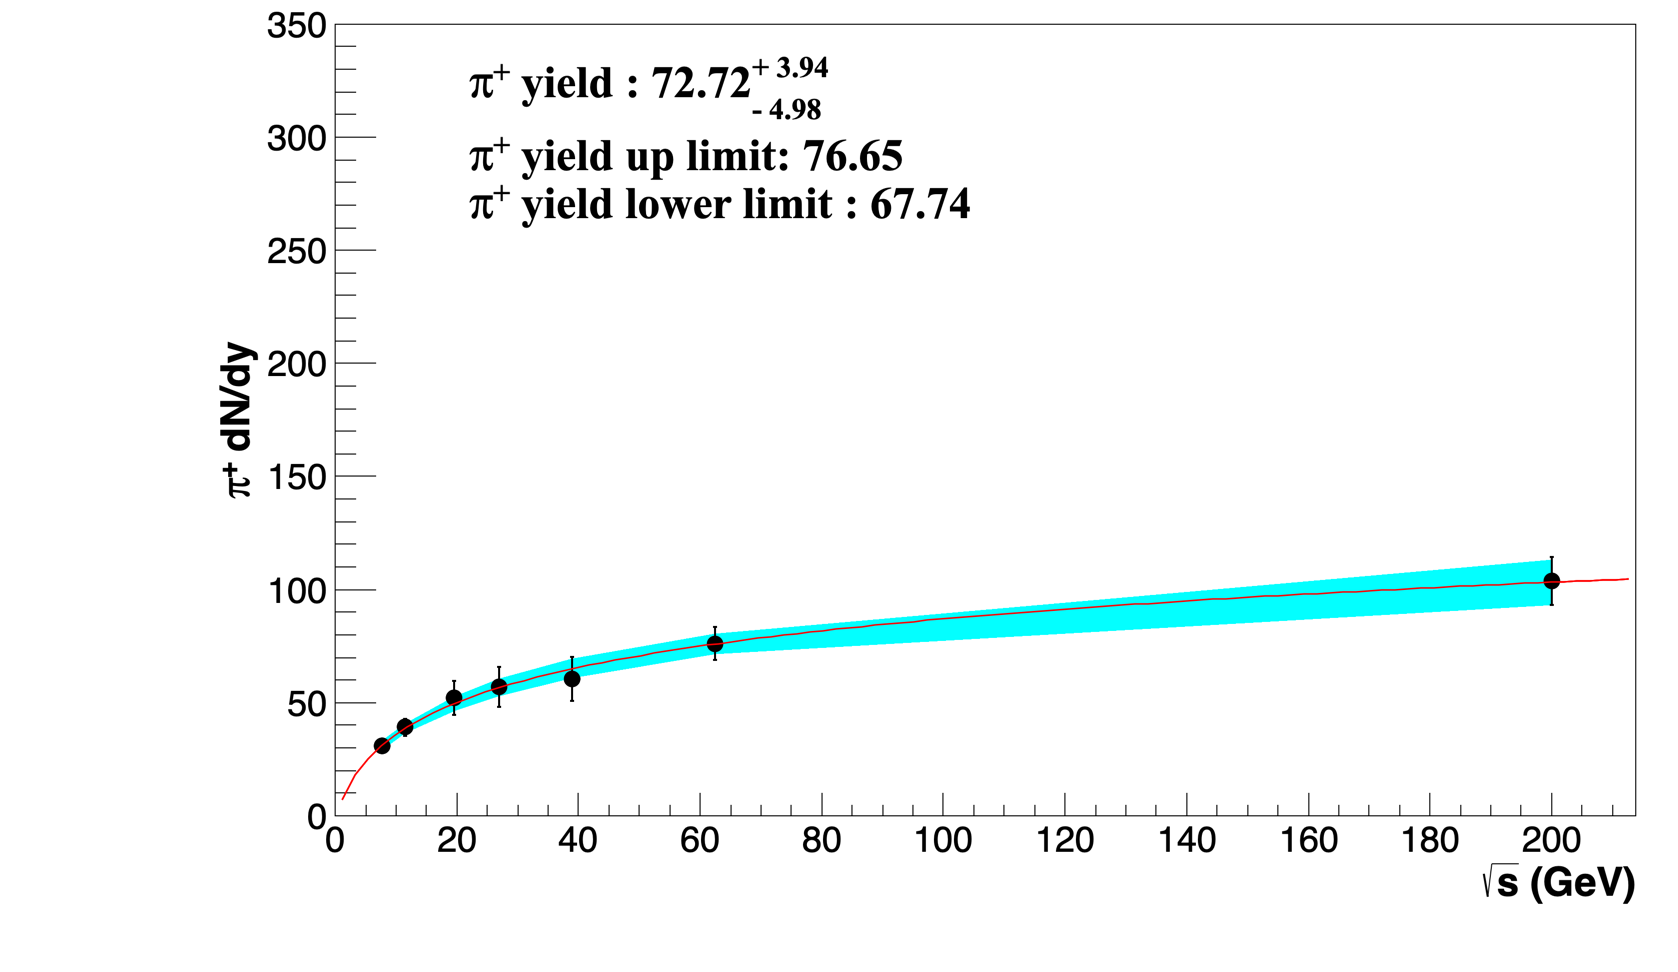
\includegraphics[width=\textwidth,clip]{figures/Chapter4/080_Plus_Yield.png}
        \caption{}
        \label{fig:pi_plus_yield}
    \end{subfigure}
    \hfill
    \begin{subfigure}[b]{0.45\textwidth}
        \centering
        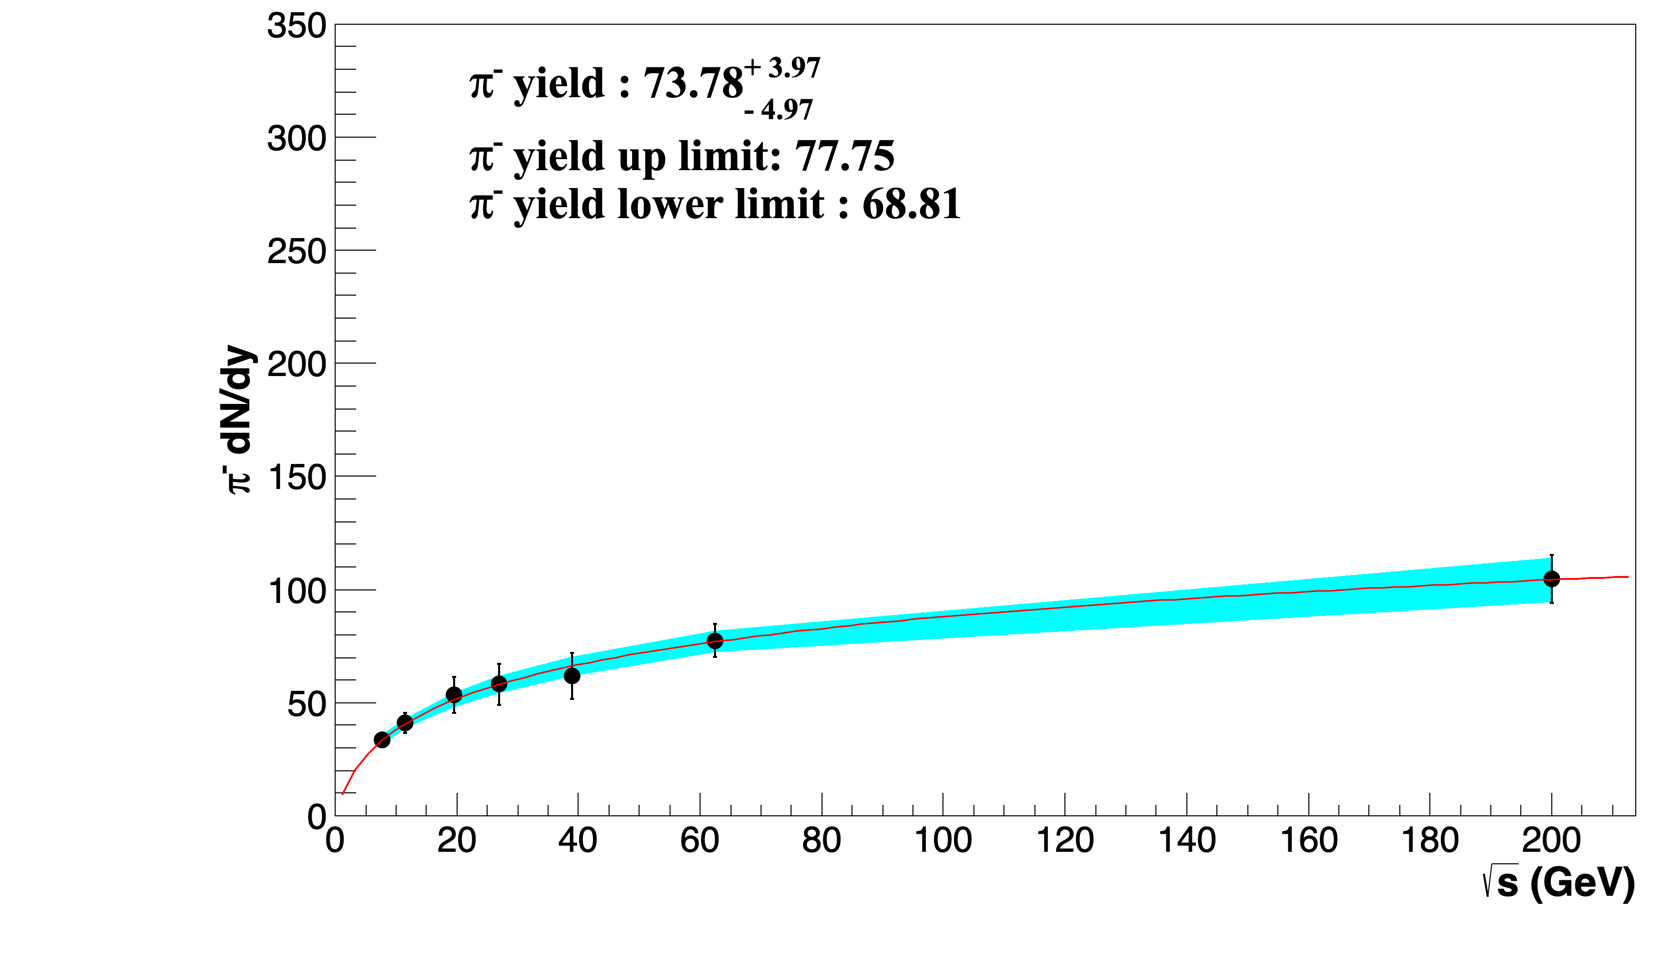
\includegraphics[width=\textwidth,clip]{figures/Chapter4/080_Minus_Yield.png}
        \caption{}
        \label{fig:pi_minus_yield}
    \end{subfigure}
    \caption[0-80\%中心度下$\pi^+$和$\pi^-$拟合的结果]{0-80\%中心度下$\pi^+$和$\pi^-$拟合的结果,左图为$\pi^+$的结果,右图为$\pi^-$的结果}
    \label{fig:pi_yield}
\end{figure}
\begin{table}[h!]
    \centering
    \caption{\sNN = 54.4 GeV 金-金对撞中不同中心度下$\pi^+$和$\pi^-$产额的值}
    \label{tab:pi_yield}
    \begin{tabularx}{0.8\textwidth} {
    | >{\centering\arraybackslash}X |>{\centering\arraybackslash}X |>{\centering\arraybackslash}X | }
        \hline
        Centrality & $\pi^+$ & $\pi^-$   \\
        \hline
        0-80\% & $72.72^{+3.94}_{-4.98}$  & $73.78^{+3.97}_{-4.97}$   \\
        \hline
        0-10\% & $203.16^{+7.60}_{-10.59}$  &  $205.87^{+7.64}_{-10.50}$  \\
        \hline
        10-40\% & $98.09^{4.06}_{5.48}$  &  $99.54^{+4.18}_{-5.55}$  \\
        \hline
        40-80\% & $21.15^{+1.21}_{-1.49}$  &  $21.49^{+1.17}_{-1.45}$  \\
        \hline
    \end{tabularx}
\end{table}

为了让最后的强子产额更加精确,在本分析当中对位于信噪比较高区间的$\omega$和$\phi$强子的产额最后是用模拟的分布去拟合真实数据抽取得到。当通过上文所述的模拟过程得到强子衰变模拟双电子谱之后,再用得到的模拟双电子谱的形状分布作为输入,对数据进行拟合。就可以得到一个额外的整体归一化因子,并用这个因子对$\omega$和$\phi$模拟谱进行归一化,使其可以更好地描述数据。在拟合的时候,整个用来拟合的强子衰变模拟的分布被分成了四部分,如式\ref{eq:float_meson}所示。其中$N_{total-\omega-\phi}$,$N_{\omega}$,$N_{\phi}$分别为总的强子衰变模拟去掉$\omega$以及$\phi$的分布、$\omega$的强子衰变模拟分布和$\phi$的强子衰变模拟分布 。$n_{broaden~\rho}$为broaden $\rho$模型中的$\rho$的分布。a、b、c、d为模拟各个分布的归一化系数。0-80\%中心度下的拟合结果如图\ref{fig:float_meson} 所示。不同中心度下的拟合参数的结果如表\ref{tab:float_meson}所示。在此拟合当中,只有$n_{\omega}$,$n_{\phi}$以及$n_{broaden~\rho}$的产额作为自由参数参与拟合,$n_{total-\omega-\phi}$被固定为1。

\begin{equation}
    \label{eq:float_meson}
    n_{fit} = a*n_{total-\omega-\phi}+b*n_{\omega}+c*n_{\phi}+d*n_{broaden~\rho}
\end{equation}

\begin{figure}[htb]
    \begin{center}
    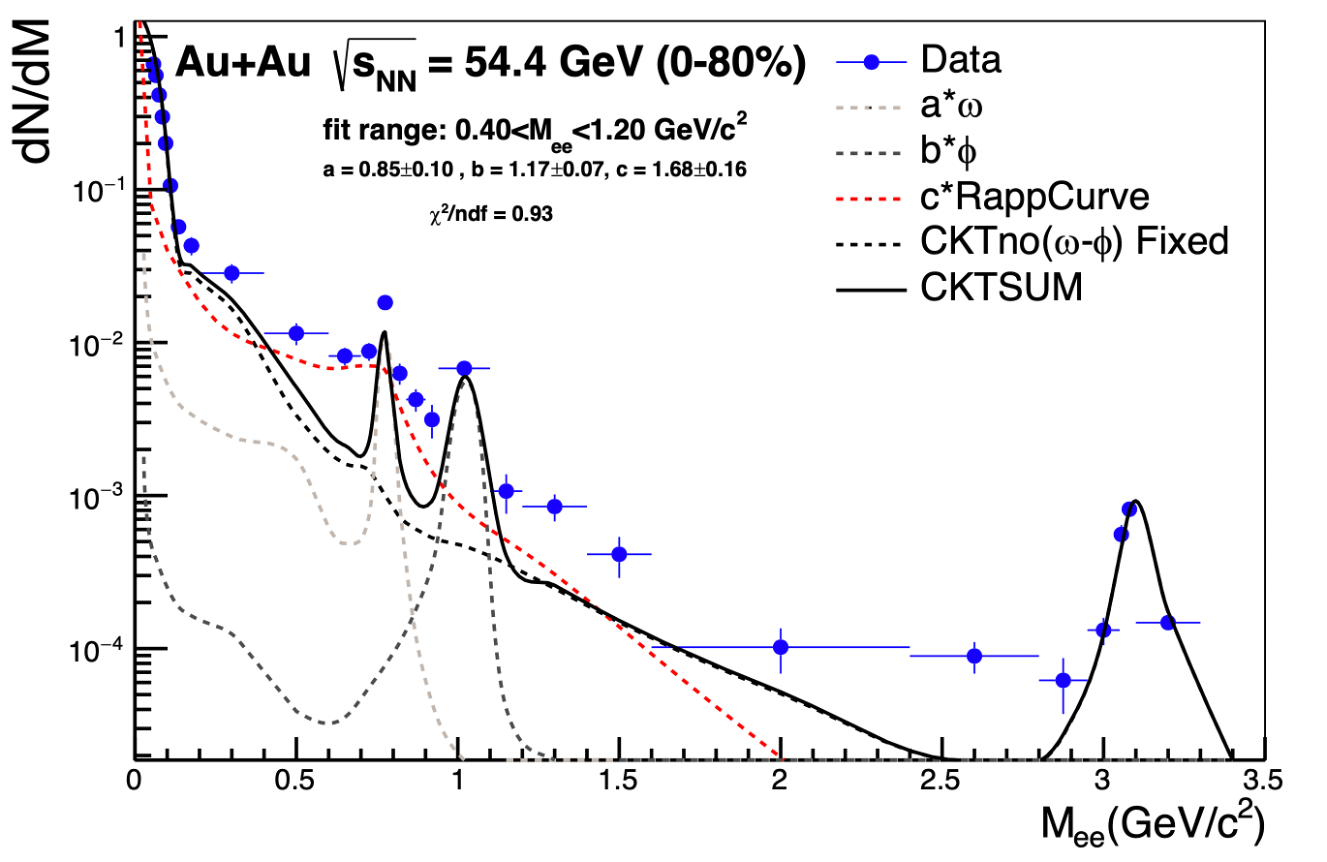
\includegraphics[width=0.75\textwidth,clip]{figures/Chapter4/float_meson.png}
    \end{center}
    \caption[强子衰变模拟对数据的拟合结果示意图]{\sNN = 54.4 GeV金-金对撞当中0-80\%中心度下强子衰变模拟对数据的拟合结果,其中蓝点为数据点,不同的拟合分量在图中用不同形式的线标出。各个分量的拟合参数已列在图中}
    \label{fig:float_meson}
\end{figure}

\begin{table}[h!]
    \centering
    \caption{54.4GeV金-金对撞中不同中心度下式\ref{eq:float_meson}中拟合参数的拟合结果}
    \label{tab:float_meson}
    \begin{tabularx}{0.8\textwidth} {
    | >{\centering\arraybackslash}X |>{\centering\arraybackslash}X |>{\centering\arraybackslash}X |>{\centering\arraybackslash}X |>{\centering\arraybackslash}X | }
        \hline
        Centrality & a & b & c & d   \\
        \hline
        0-80\%  & 1 & $0.85 \pm 0.10$ & $1.17 \pm 0.07$ & $1.68 \pm 0.16$ \\
        \hline
        0-10\%  & 1 & $0.90 \pm 0.20$ & $1.35 \pm 0.17$ & $1.42 \pm 0.27$ \\
        \hline
        10-40\% & 1 & $0.86 \pm 0.10$ & $1.14 \pm 0.08$ & $1.53 \pm 0.17$ \\
        \hline
        40-80\% & 1 & $1.05 \pm 0.09$ & $1.07 \pm 0.07$ & $2.58 \pm 0.20$ \\
        \hline
    \end{tabularx}
\end{table}

